\section{Solution theory}

As we have seen above, we cannot rule out the emergence of discontinuities for conservation laws. We thus need a ``weaker'' solution concept to make sense of these PDEs for discontinuous solutions.


\subsection{Weak solution}

\begin{definition}
	Let \(u: \R \times \parentheses*{0, \infty} \to \R\) be locally integrable, i.e., \(u \in L_{\text{loc}}^1\parentheses*{\R \times \parentheses*{0, \infty}}\).
	Then \(u\) is called a \emph{weak solution} of the conservation law with initial value \(u_0 \in L_{\text{loc}}^1\parentheses*{\R}\), if it satisfies
	\[
		\int_0^\infty \int_\R \parentheses*{u\partial_t \varphi + f\parentheses*{u}\partial_x \varphi}\d x\d t + \int_\R u_0\parentheses*{x}\varphi\parentheses*{x, 0}\d x = 0 \quad \forall \varphi \in C_0^1\parentheses*{\R \times \left[0, \infty\right)}.
	\]
\end{definition}

\begin{remark}
	\begin{enumerate}
		\item Notice that test functions \(\varphi \in C_0^1\parentheses*{\R \times \left[0, \infty\right)}\) are sufficient for conservation laws, because they are first order PDEs.
		One could, of course, equivalently use \(C_0^\infty\parentheses*{\R \times \left[0, \infty\right)}\) instead, in view of the density of \(C_0^\infty\parentheses*{\R \times \left[0, \infty\right)} \subset \C_0^1\parentheses*{\R \times \left[0, \infty\right)}\), which would then mimic the ideas for deriving weak solutions for elliptic PDEs more closely.
		\item Similarly, one could also use \(C_0^1\parentheses*{\R^2}\) (or \(C_0^\infty\parentheses*{\R^2}\)) as test functions, i.e., test functions \(\varphi\) defined on the entire \(xt\)-plane with \(\varphi \to 0\) as \(\absolute*{t}, \absolute*{x} \to \infty\), because the integration limits then localize these functions to the relevant subdomain \(\R \times \R^+\).
		\item Observe that the initial condition is only weakly enforced.
	\end{enumerate}
\end{remark}

\begin{theorem}
	\begin{enumerate}
		\item Ever classical, or strong, (i.e., differentiable) solution is also a weak solution.
		\item If \(u\) is a weak solution satisfying \(u \in C^1\parentheses*{\R \times \R^+}\), then \(u\) is also a strong (i.e., classical) solution.
	\end{enumerate}
\end{theorem}

\begin{proof}
	\begin{enumerate}
		\item Let \(u \in C^1\parentheses*{\R \times \R^+}\) solve \(\partial_t u + \partial_x f\parentheses*{u} = 0\) in \(\R\) for \(t > 0\), and \(u\parentheses*{x, 0} = u_0\parentheses*{x}\).
		For \(R > 0\) we choose a domain \(\Omega_R := \braces*{\parentheses*{x, t} \in \R \times \R + : x^2 + t^2 < R^2} \subset \R \times \R^+\) as depicted.
		\begin{center}
			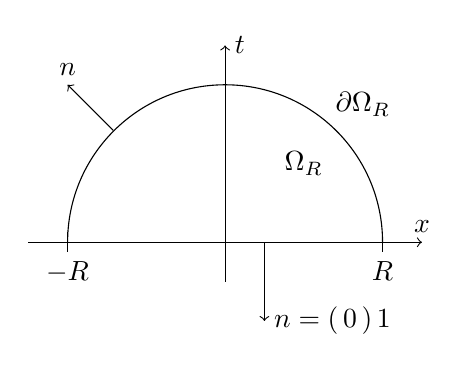
\begin{tikzpicture}
				\draw[->] (-2.5,0) -- (2.5,0) node[above] {\(x\)};
				\draw[->] (0,-.5) -- (0,2.5) node[right] {\(t\)};
				\begin{scope}
					\clip (-2.5,0) rectangle (2.5,2.5);
					\draw (0,0) circle (2);
				\end{scope}
				\draw[->] (.5,0) -- (.5,-1) node[right] {\(n = \begin{pmatrix}
					0\\
					1
				\end{pmatrix}\)};
				\draw (-2,.125) -- (-2,-.125) node[below] {\(-R\)};
				\draw (2,.125) -- (2,-.125) node[below] {\(R\)};
				\node at (1,1) {\(\Omega_R\)};
				\node at (1.75,1.75) {\(\partial\Omega_R\)};
				\draw[->] (-1.42,1.42) -- (-2,2) node[above] {\(n\)};
			\end{tikzpicture}
		\end{center}
		For any test function \(\varphi \in C_0^1\parentheses*{\R \times \left[0, \infty\right)}\) we multiply the PDE by \(\varphi\) and integrate to find
		\begin{align*}
			0 &= \int_{\R \times \R^+}\parentheses*{\partial_t u + \partial_x f\parentheses*{u}}\varphi\d x\d t\\
			&= \lim_{R \to \infty}\parentheses*{\int_{\Omega_R}\parentheses*{\partial_t\parentheses*{u\varphi} + \partial_x\parentheses*{f\parentheses*{u}\varphi}}\d x\d t - \int_{\Omega_R} \parentheses*{u\partial_t \varphi + f\parentheses*{u}\partial_x \varphi}\d x\d t}.
		\end{align*}
		The first integrand can be identified as a divergence in \(\parentheses*{x, t}\), for which the Gauss theorem yields
		\begin{align*}
			\int_{\Omega_R}\parentheses*{\partial_t \parentheses*{u\varphi} + \partial_x \parentheses*{f\parentheses*{u}\varphi}}\d x\d t &= \int_{\Omega_R}\div_{\parentheses*{x, t}}\begin{pmatrix}
				f\parentheses*{u}\varphi\\
				u\varphi
			\end{pmatrix}\d x\d t\\
			&= \int_{\partial\Omega}\begin{pmatrix}
				f\parentheses*{u}\varphi\\
				u\varphi
			\end{pmatrix} \cdot n\d l\\
			&= \int_{\Gamma_R}\varphi\begin{pmatrix}
				f\parentheses*{u}\\
				u
			\end{pmatrix} \cdot n\d l + \int_{\Gamma_0}\varphi\begin{pmatrix}
				f\parentheses*{u}\\
				u
			\end{pmatrix} \cdot \begin{pmatrix}
				0\\
				-1
			\end{pmatrix}\d l,
		\end{align*}
		where we have decomposed the boundary of \(\Omega_R\) as \(\partial\Omega_R = \Gamma_0 \cup \Gamma_R\) with \(\Gamma_0 := \braces*{\parentheses*{x, 0} : -R < x < R}\) and \(\Gamma_R = \partial\Omega_R \setminus \Gamma_0\).
		As the test function vanishes on \(\Gamma_R\) for \(R \to \infty\) due to its compact support, we find that the boundary integral over \(\Gamma_R\) vanishes.
		Consequently, we obtain
		\begin{align*}
			0 &= \lim_{R \to \infty}\parentheses*{\int_{\Omega_R} \parentheses*{\partial_t \parentheses*{u\varphi} + \partial_x\parentheses*{f\parentheses*{u}\varphi}}\d x\d t - \int_{\Omega_R}\parentheses*{u\partial_t \varphi + f\parentheses*{u}\partial_x \varphi}\d x\d t}\\
			&= -\lim_{R \to \infty}\parentheses*{\int_{-R}^R \varphi\parentheses*{x, 0}u_0\parentheses*{x}\d x + \int_{\Omega_R}\parentheses*{u\partial_t \varphi + f\parentheses*{u}\partial_x \varphi}\d x\d t}\\
			&= \int_0^\infty \int_\R \parentheses*{u\partial_t \varphi + f\parentheses*{u}\partial_x \varphi}\d x\d t + \int_\R \varphi\parentheses*{x, 0}u_0\parentheses*{x}\d x,
		\end{align*}
		for any \(\varphi \in C_0^1\parentheses*{\R \times \left[0, \infty\right)}\).
		\item This follows analogously by using the arguments ``backwards'', which requires \(u\) to be differentiable.
	\end{enumerate}
\end{proof}
